\documentclass[tikz,border=2pt]{standalone}
\usepackage{amsmath,amssymb}
\usepackage{tikz}
\usetikzlibrary{arrows.meta}

\begin{document}
% Means add: X takes 1 or 3 (mean 2), Y takes 2 or 6 (mean 4), and whatever the dependence
% between them the mean of X + Y is 6 = 2 + 4.
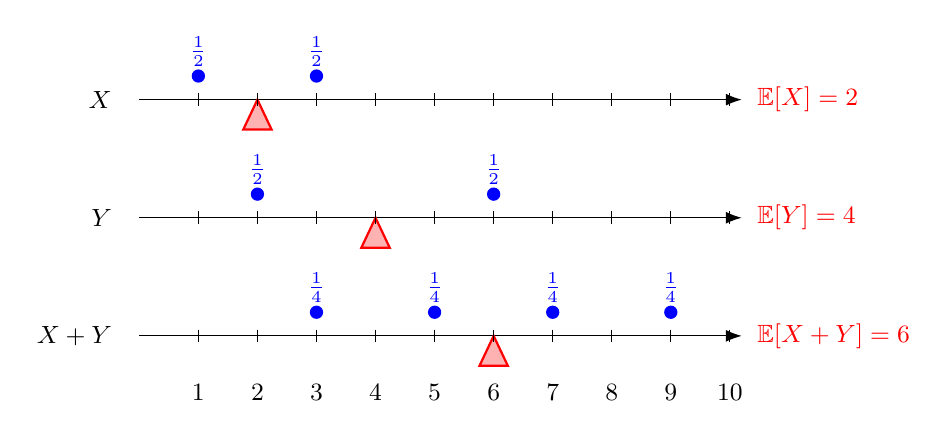
\begin{tikzpicture}[x=0.75cm, every node/.style={font=\small}, >={Latex[length=2mm]}]
	\foreach \row/\lab/\mean in {0/$X$/2, -1.5/$Y$/4, -3.0/$X+Y$/6} {
		\draw[->] (0,\row) -- (10.2,\row);
		\node[anchor=east] at (-0.3,\row) {\lab};
		\draw[red, thick, fill=red!30] (\mean,\row) -- ({\mean-0.24},{\row-0.38}) -- ({\mean+0.24},{\row-0.38}) -- cycle;
	}
	\foreach \x in {1,...,10} {\draw (\x,0.08) -- (\x,-0.08); \draw (\x,-1.42) -- (\x,-1.58); \draw (\x,-2.92) -- (\x,-3.08); \node[below=14pt] at (\x,-3.0) {\x};}
	\fill[blue] (1,0.3) circle (2.4pt) node[above] {$\tfrac12$};
	\fill[blue] (3,0.3) circle (2.4pt) node[above] {$\tfrac12$};
	\fill[blue] (2,-1.2) circle (2.4pt) node[above] {$\tfrac12$};
	\fill[blue] (6,-1.2) circle (2.4pt) node[above] {$\tfrac12$};
	\foreach \x in {3,5,7,9} {\fill[blue] (\x,-2.7) circle (2.4pt) node[above] {$\tfrac14$};}
	\node[red, anchor=west] at (10.3,0) {$\mathbb{E}[X]=2$};
	\node[red, anchor=west] at (10.3,-1.5) {$\mathbb{E}[Y]=4$};
	\node[red, anchor=west] at (10.3,-3.0) {$\mathbb{E}[X+Y]=6$};
	
\end{tikzpicture}
\end{document}
